\section{Method}

\label{sec:methodology}

\subsection{Overview}

The method stores a graph $G_t$ and rules $R_t$. At each step, a policy
gets rules, removes rules, or repairs the graph with an active rule.
New rules can allow later repairs. Remaining errors guide the choice
of further rules. A fixed budget limits the actions.

Figure~\ref{fig:rl_framework} shows the scheduling loop.
Figure~\ref{fig:dual_strategy} shows the two rule prompts.
The scheduling test uses a fixed rule library. Further tests compile
saved candidates and run them through a repair interface. Document tests
get one response at a time and check source rules.

\subsection{Quality Scores}

\label{subsec:quality_model}

\subsubsection{Graph Quality}

After each graph action, code counts isolated nodes, repeated edges,
invalid relations, and edges with missing endpoints. Their rates are
$I_r,D_r,V_r,L_r$. The four quality scores are

\begin{equation}
\begin{aligned} S(C_1)&=1-I_r,& S(C_2)&=1-D_r,\\ S(C_3)&=1-V_r,& S(C_4)&=1-L_r.\end{aligned}
\end{equation}

The test uses

\begin{equation}
\label{eq:kg_quality}
Q(G)=0.20S(C_1)+0.20S(C_2)+0.30S(C_3)+0.30S(C_4).
\end{equation}

These fixed weights define the structural quality score.

\subsubsection{Rule Quality}

We score active rules on a fixed set of 180 calibration cases.
This set is stored apart from the graph corruption list.
The union of rule predictions gives

\begin{equation}
\Precision(R)=\frac{TP}{TP+FP},\qquad \Recall(R)=\frac{TP}{TP+FN}.
\end{equation}

An empty rule set has zero precision and recall. Coverage is the share
of four error families with an active rule. The online score is

\begin{equation}
\label{eq:qr_online}
\begin{aligned}Q_{\mathrm{online}}(R)={}&0.35\Precision(R)+0.35\Recall(R)\\&+0.30\Coverage(R).\end{aligned}
\end{equation}

Each high-precision module detects 27 of 30 family-positive cases and
two clean cases in the calibration set. Three more modules have lower
precision. Rule scores use this fixed set. Generation tests count candidates
from saved responses.

\subsection{Learning to Choose Graph and Rule Actions}

\label{subsec:rl_co_optimization}

\subsubsection{Environment and Policy Inputs}

The state stores the graph, active rules, budget, initial error counts,
and trusted relation-restoration records. The environment holds these
restoration records. The policy receives fourteen values:

\begin{equation}
\begin{split}
o_t=[&S(C_1),S(C_2),S(C_3),S(C_4),\\
&\Precision,\Recall,\Coverage,\tilde n_{\mathrm{iso}},\tilde n_{\mathrm{dup}},\\
&\tilde n_{\mathrm{invalid}},\tilde n_{\mathrm{dang}},\tilde b,\rho_{\mathrm{valid}},\rho_{\mathrm{noisy}}]_t.
\end{split}
\end{equation}

We divide each error count by its episode-initial count, using at least
one as the denominator. The last entries give the remaining budget share
and active shares of high- and low-precision modules. Each input value
is clipped to $[0,1.5]$. Coverage equals $\rho_{\mathrm{valid}}$ in this
library. Both inputs remain in the shared network design. The network
uses these fourteen values and the action mask.

The eight actions are

\begin{equation}
\begin{split}
\mathcal A=\{&a_{\mathrm{iso}},a_{\mathrm{dup}},a_{\mathrm{rel}},a_{\mathrm{dang}},\\
&a_{\mathrm{del}},a_{\mathrm{aug}},a_{\mathrm{mix}},a_{\mathrm{prune}}\}.
\end{split}
\end{equation}

The first four actions remove isolated noise nodes, remove duplicate
edges, restore invalid relation names, and remove edges with missing
endpoints. Each handles a batch based on 60\% of the remaining matching
errors. Relation repair uses the private corruption record after detection.

The other actions activate a deletion module, activate an augmentation
module, activate one module from each family, or remove modules with
calibration precision below 0.5. Acquisition follows the fixed library
order. Repair requires an active rule and a matching error. These actions
activate stored modules. The text prompts below supply candidates for
further execution tests.

The graph and active rule IDs determine the action mask. All compared
policies receive this mask, except the no-mask setting. Policies receive
the current inputs and mask. A separate model-informed baseline can copy
the environment and try future actions.

\subsubsection{Reward and Double DQN}

The reward uses $\Delta Q(G_t)=Q(G_{t+1})-Q(G_t)$ and the change in rule
score. It subtracts costs for acquisition, edits, and new errors:

\begin{equation}
\label{eq:reward_def}
\begin{split}
r_t={}&\Delta Q(G_t)+0.4\Delta Q_{\mathrm{online}}(R_t)\\
&-0.004C_{\mathrm{call}}-2\times10^{-5}C_{\mathrm{edit}}-P_t.
\end{split}
\end{equation}

$C_{\mathrm{call}}$ counts one unit for single-family acquisition and
two for mixed acquisition. These units measure simulated call cost.
Pruning has zero call cost. The environment computes $N_{\mathrm{new}}$
from error IDs before and after the action. Each node and edge copy has
its own fixed ID. The edit count includes graph changes and active-rule
changes. Logs also give these two counts apart.

An episode ends when $Q(G)\geq0.999$ and $Q_{\mathrm{online}}(R)\geq0.90$,
after 18 decisions, or when no action is allowed. An action that would
empty a nonempty node or edge set is undone and ends the episode.

Let $\mathcal V(G)$ be the multiset of detected error IDs. Then

\begin{equation}
N_{\mathrm{new}}=\left|\mathcal V(G_{t+1})\setminus_{\!m}\mathcal V(G_t)\right|,
\end{equation}

Here $\setminus_m$ is multiset difference. Removing an edge with a missing
endpoint can leave its other endpoint isolated. One old error disappears
and a new one appears. The total count can stay the same. The new term
charges for the new error. Each step saves its new error IDs and reward parts.

We compare three fixed choices of $P_t$. Let $n_{k,t}$ count new error IDs
in family $k$. Let $w_k$ be the weight in Equation~\ref{eq:kg_quality}.
The penalties are

\begin{equation}
\label{eq:safety_modes}
\begin{aligned}
P_t^{\mathrm{count}}&=0.01\sum_k n_{k,t},\\
P_t^{\mathrm{rate}}&=\sum_k w_k\frac{n_{k,t}}{D_{k,0}},\qquad
P_t^{\mathrm{zero}}=0,\\
D_{k,0}&=\begin{cases}
\max(1,|V_0|),&k=\text{isolation},\\
\max(1,|E_0|),&\text{otherwise}.
\end{cases}
\end{aligned}
\end{equation}

$V_0$ and $E_0$ are the nodes and edge copies after initial corruption.
The denominators stay fixed during the episode. The rate penalty divides
new error counts by the initial graph size. Call and edit costs keep their
fixed weights. All three settings share inputs, masks, and graph operations.
A duplicate edge can repeat a correct fact. We score structural errors
and wrong facts apart.

For $J_t=Q(G_t)+0.4Q_{\mathrm{online}}(R_t)$, discounted quality gains satisfy

\begin{equation}
\begin{split}
\sum_{t=0}^{T-1}\gamma^t(J_{t+1}-J_t)
={}&-J_0+\gamma^{T-1}J_T\\
&+(1-\gamma)\sum_{t=1}^{T-1}\gamma^{t-1}J_t.
\end{split}
\end{equation}

The policy thus values early gains and final quality.

A deep Q-network (DQN) predicts the value of each action.
We use DQN~\cite{mnih2015human} with the Double-DQN target~\cite{vanhasselt2016deep}.
The online Q-network has layers $14\rightarrow32\rightarrow16\rightarrow8$
and ReLU activations. The replay buffer stores $(o_t,a_t,r_t,o_{t+1},d_t)$
and the next-action mask. For a nonempty next-action set, $a^*$ chooses
the highest online-network value. The target is

\begin{equation}
\begin{aligned}
a^*&=\arg\max_{a'\in\mathcal A_{t+1}}Q(o_{t+1},a';\theta),\\
y_t&=\begin{cases}
r_t,&d_t=1\text{ or }\mathcal A_{t+1}=\emptyset,\\
r_t+\gamma Q(o_{t+1},a^*;\theta^-),&\text{otherwise},
\end{cases}\\
\mathcal L(\theta)&=\mathbb E[\operatorname{Huber}(Q(o_t,a_t;\theta)-y_t)].
\end{aligned}
\end{equation}

The bootstrap term is zero at a terminal state or an empty allowed set.
We copy target parameters every 100 environment steps. Standard DQN uses
$\max_{a'}Q(o_{t+1},a';\theta^-)$ as its next-state target.

Adam uses learning rate $0.002$ and discount $0.95$. Replay capacity is
20,000, batch size is 64, and warm-up is 128 transitions. Each model trains
for 250 episodes. Exploration falls linearly over 260 episodes.
The last training episode uses $\epsilon\approx0.0902$; the lower limit
is 0.05. The reward study saves ten checkpoints per setting: Double DQN
with count, rate, or zero penalty, and DQN with rate penalty.
Appendix~\ref{app:impl} gives the earlier sixty-model count-penalty study.
Training runs in the local environment with zero API calls.

\subsection{Generating Rules with Two Prompts}

\label{subsec:llm_rule}

The two prompts propose rules from source text. Each uses one call per
document and strategy. The JSON response contains entity types, relation
types, allowed and forbidden type patterns, hierarchy statements,
geographical hierarchy patterns, and statements about required steps.
Equal-budget tests count type declarations and constraints apart.

\subsubsection{Deletion Completion}

\label{subsubsec:deletion}

The code replaces short text spans with missing-span markers.
By default, it chooses up to five start points and at most six characters
per span. The prompt includes the original text, changed text, removed
spans, and shared JSON format. It asks for missing rule information and
reusable constraints. The model compares both versions.

\begin{algorithm}[t]
\caption{Deletion-completion steps}
\label{alg:deletion_completion}
\begin{algorithmic}[1]
\Require Document ID $d$, source text $T$
\State $(T^-,F)\leftarrow\operatorname{DeleteShortSpans}(T)$
\State $P\leftarrow\operatorname{DeletionPrompt}(T,T^-,F)$
\State $Y\leftarrow\operatorname{LLM}(P)$ \Comment{One call}
\State Parse the JSON candidate categories in $Y$
\State Log $(d,\text{deletion},F,Y)$
\State \Return grouped candidates, including parse status
\end{algorithmic}
\end{algorithm}

\subsubsection{Augmentation Expansion}

\label{subsubsec:augmentation}

The augmentation prompt includes the source and asks for up to three
reasonable extra sentences. The same response gives rules from these sentences.
The sentences guide the search for further candidates.

\begin{algorithm}[t]
\caption{Augmentation-expansion steps}
\label{alg:augmentation_expansion}
\begin{algorithmic}[1]
\Require Document ID $d$, source text $T$
\State $P\leftarrow\operatorname{AugmentationPrompt}(T)$
\State $Y\leftarrow\operatorname{LLM}(P)$ \Comment{Sentences and candidates in one call}
\State Parse the JSON candidate categories in $Y$
\State Log $(d,\text{augmentation},Y)$
\State \Return grouped candidates, including parse status
\end{algorithmic}
\end{algorithm}

\begin{figure*}[t]
\centering
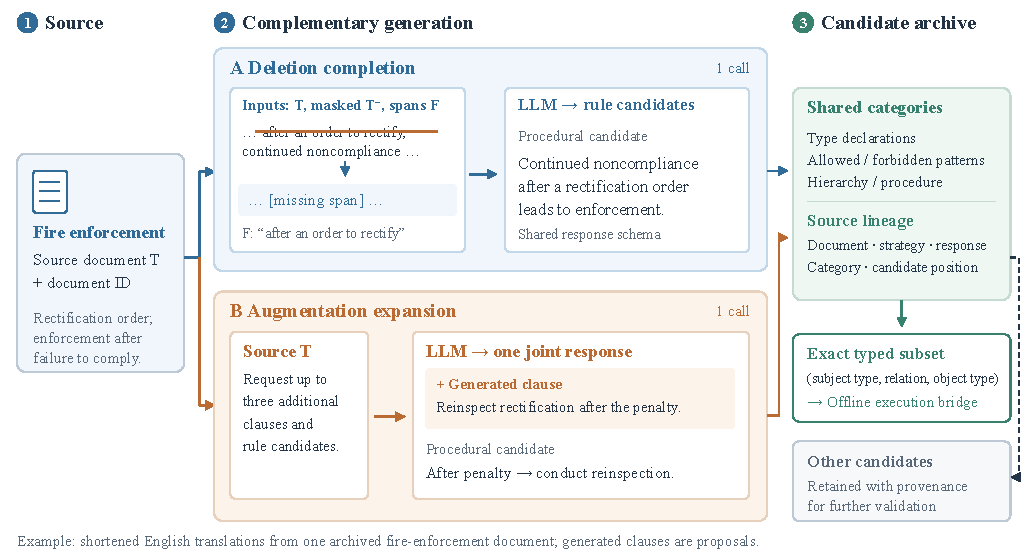
\includegraphics[width=0.96\textwidth]{figure/method/dual_strategy.pdf}
\caption{Two rule prompts, with short English examples from a saved fire-enforcement document. Deletion receives original text, changed text, and removed spans. Augmentation returns extra sentences and candidates in one response. Each candidate keeps its source record. Exact type patterns enter the repair interface.}
\label{fig:dual_strategy}
\end{figure*}

\subsubsection{Compiling and Checking Rules}

\label{subsubsec:rule_materialization}

We save each candidate's document, strategy, response line, category,
and position. The compiler supports exact subject-type, relation,
and object-type triples. A forbidden pattern $r=(\tau_s,p,\tau_o)$ flags
a record $x$ when

\begin{equation}
V_r(x)=\mathbf1[(\operatorname{type}(s_x),p_x,\operatorname{type}(o_x))=r].
\end{equation}

An allowed pattern permits that exact combination.
A record is flagged by a matching forbidden rule. If both kinds match,
the checker records a conflict and skips the decision. It trims spaces
at the ends of strings and matches the remaining text exactly.

The log keeps malformed candidates, unsupported families, unmapped terms,
and patterns with zero matches. RuleTest-94 supplies stored expected
outcomes for execution tests. Hand-written checks for required steps
and structural errors form a separate comparison.

\subsubsection{Removing Copies and Saving Sources}

The saved code removes identical candidates within each category using
a fixed text format. It counts entity and relation declarations apart
from constraints.

The generation script defaults to Qwen3-32B and temperature 0.2.
Historical call records store parsed outputs and document information.
Appendix~\ref{app:prompts} gives the prompt builders, translations,
and recorded settings. The supplement supplies the literal templates.
The separate extraction test uses Qwen3.8-27B-no-thinking.

\subsection{Repair with Saved Generated Rules}

\label{sec:rule_bridge_method}

The repair interface compiles saved allowed and forbidden type patterns
with the same exact-match rule. Activation updates the error report.
A forbidden rule with no matching allowed rule allows record removal.
After removal, the interface checks matches and allowed actions again.
Each match saves its rule ID and original source. Unsupported candidates
are logged. Conflicting patterns cause the checker to skip the decision.

The replay adapter provides reset, observation, available-action, and step
functions. Its four commands load deletion rules, load augmentation rules,
remove forbidden matches, or stop. The policy sees record, flag, conflict,
and active-rule counts, acquisition status, budget, and mask.
Each bank loads once. Stop or six decisions end replay. This adapter
runs fixed schedules. The eight-action environment supplies training rewards.

Missing endpoints or unknown types cause the checker to skip a record.
A allowed rule arriving after removal is logged against that removed record.
A removal that would empty a nonempty set is blocked. Logs save activations,
detections, removals, and their sources. The scorer reads reference labels.
Removing a record leaves it absent. Loading a full saved bank has its own
acquisition count.

\paragraph{Document development environment.}

The document environment gets one saved response at a time. Its four
actions acquire deletion, acquire augmentation, repair, and stop.
An episode allows four responses and ten decisions. The reward counts
errors found by new rules apart from errors created by edits
(Appendix~\ref{app:docred_v2}). Fixed schedules and all-path replay measure
repair coverage. Eight-action checkpoints run in their original rule library.

\paragraph{Rule approval for each document.}

The admission layer links each candidate to its response, source documents,
initial records, and relation vocabulary. A rule needs valid source links
and approval from the chosen review channel. It becomes active when its
response is acquired. Permissions, support rules, and forbidden rules share
this requirement. Type review covers all initial matching records in
the document pair. New or changed records need new review.
Model judgments and independent reviews have separate channels.
